\documentclass[final]{beamer}
\usepackage[scale=1.24]{beamerposter}
\usepackage{graphicx,booktabs} 
\usepackage{helvet}

\usetheme{confposter}
\setbeamercolor{block title}{fg=Maroon,bg=white}
\setbeamercolor{block body}{fg=black,bg=white}
\setbeamercolor{block alerted title}{fg=white,bg=Maroon!70}
\setbeamercolor{block alerted body}{fg=black,bg=Maroon!10} 

\newlength{\sepwid}
\newlength{\onecolwid}
\newlength{\twocolwid}
\newlength{\threecolwid}
\setlength{\paperwidth}{48in}
\setlength{\paperheight}{36in}
\setlength{\sepwid}{0.024\paperwidth}
\setlength{\onecolwid}{0.22\paperwidth}
\setlength{\twocolwid}{0.464\paperwidth}
\setlength{\threecolwid}{0.708\paperwidth}
\setlength{\topmargin}{-0.5in}

\title{Fido: A Universal Robot Control System using\\Reinforcement Learning with Limited Feedback}
\author{Joshua Gruenstein \and Michael Truell}
\institute{Horace Mann School}

\begin{document}

\addtobeamertemplate{block end}{}{\vspace*{2ex}}
\addtobeamertemplate{block alerted end}{}{\vspace*{2ex}}
\setlength{\belowcaptionskip}{2ex}
\setlength\belowdisplayshortskip{2ex}

\begin{frame}[t]
\begin{columns}[t]

\begin{column}{\sepwid}\end{column}
\begin{column}{\onecolwid}

	\begin{alertblock}{Control System Objectives}
		Fido was created to fulfill the following goals:
		\begin{itemize}
			\item \textbf{Trainability}: Allow both human and autonomous training rather than reprogramming
			\item \textbf{Universality}: Run on any robot, even without prior knowledge of the host
		\end{itemize}
		These goals were achieved through the training of artificial neural networks with a wire-fitted moving least squares interpolator following the Q-learning reinforcement algorithm and an action selection policy that utilizes a Boltzmann distribution of probability.
	\end{alertblock}

	\begin{block}{Implementation}
		Fido was programmed in C++, with no external dependencies.  However, the simulator does use the SFML graphics library.  The hardware implementation uses the Intel Edison embedded platform, a 3D printed chassis and a differential drive system.

		\begin{figure}
			\centering
			\fbox{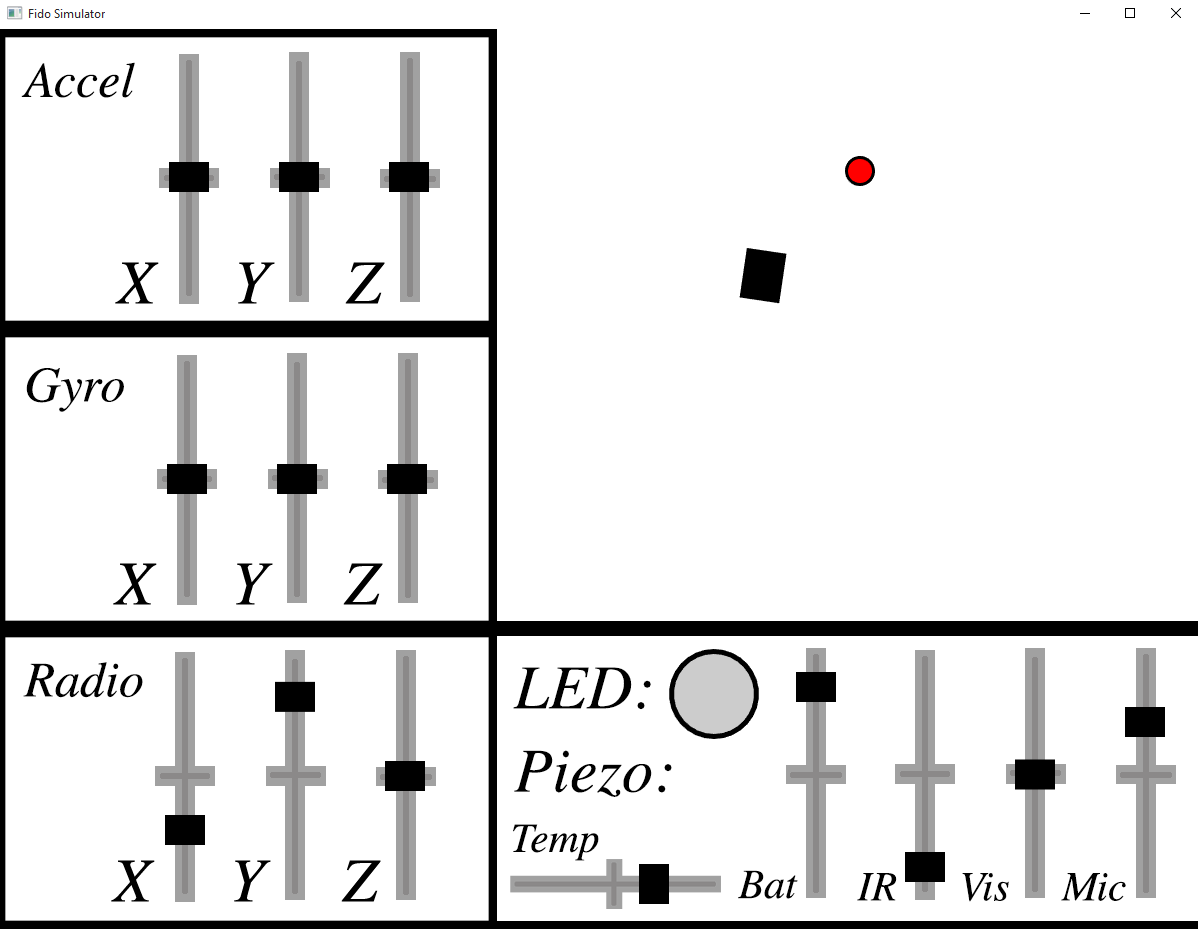
\includegraphics[width=.75\linewidth]{Figures/Screenshot.png}}
			\caption{Fido Simulator Graphical User Interface}
		\end{figure}

		\begin{figure}
			\centering
			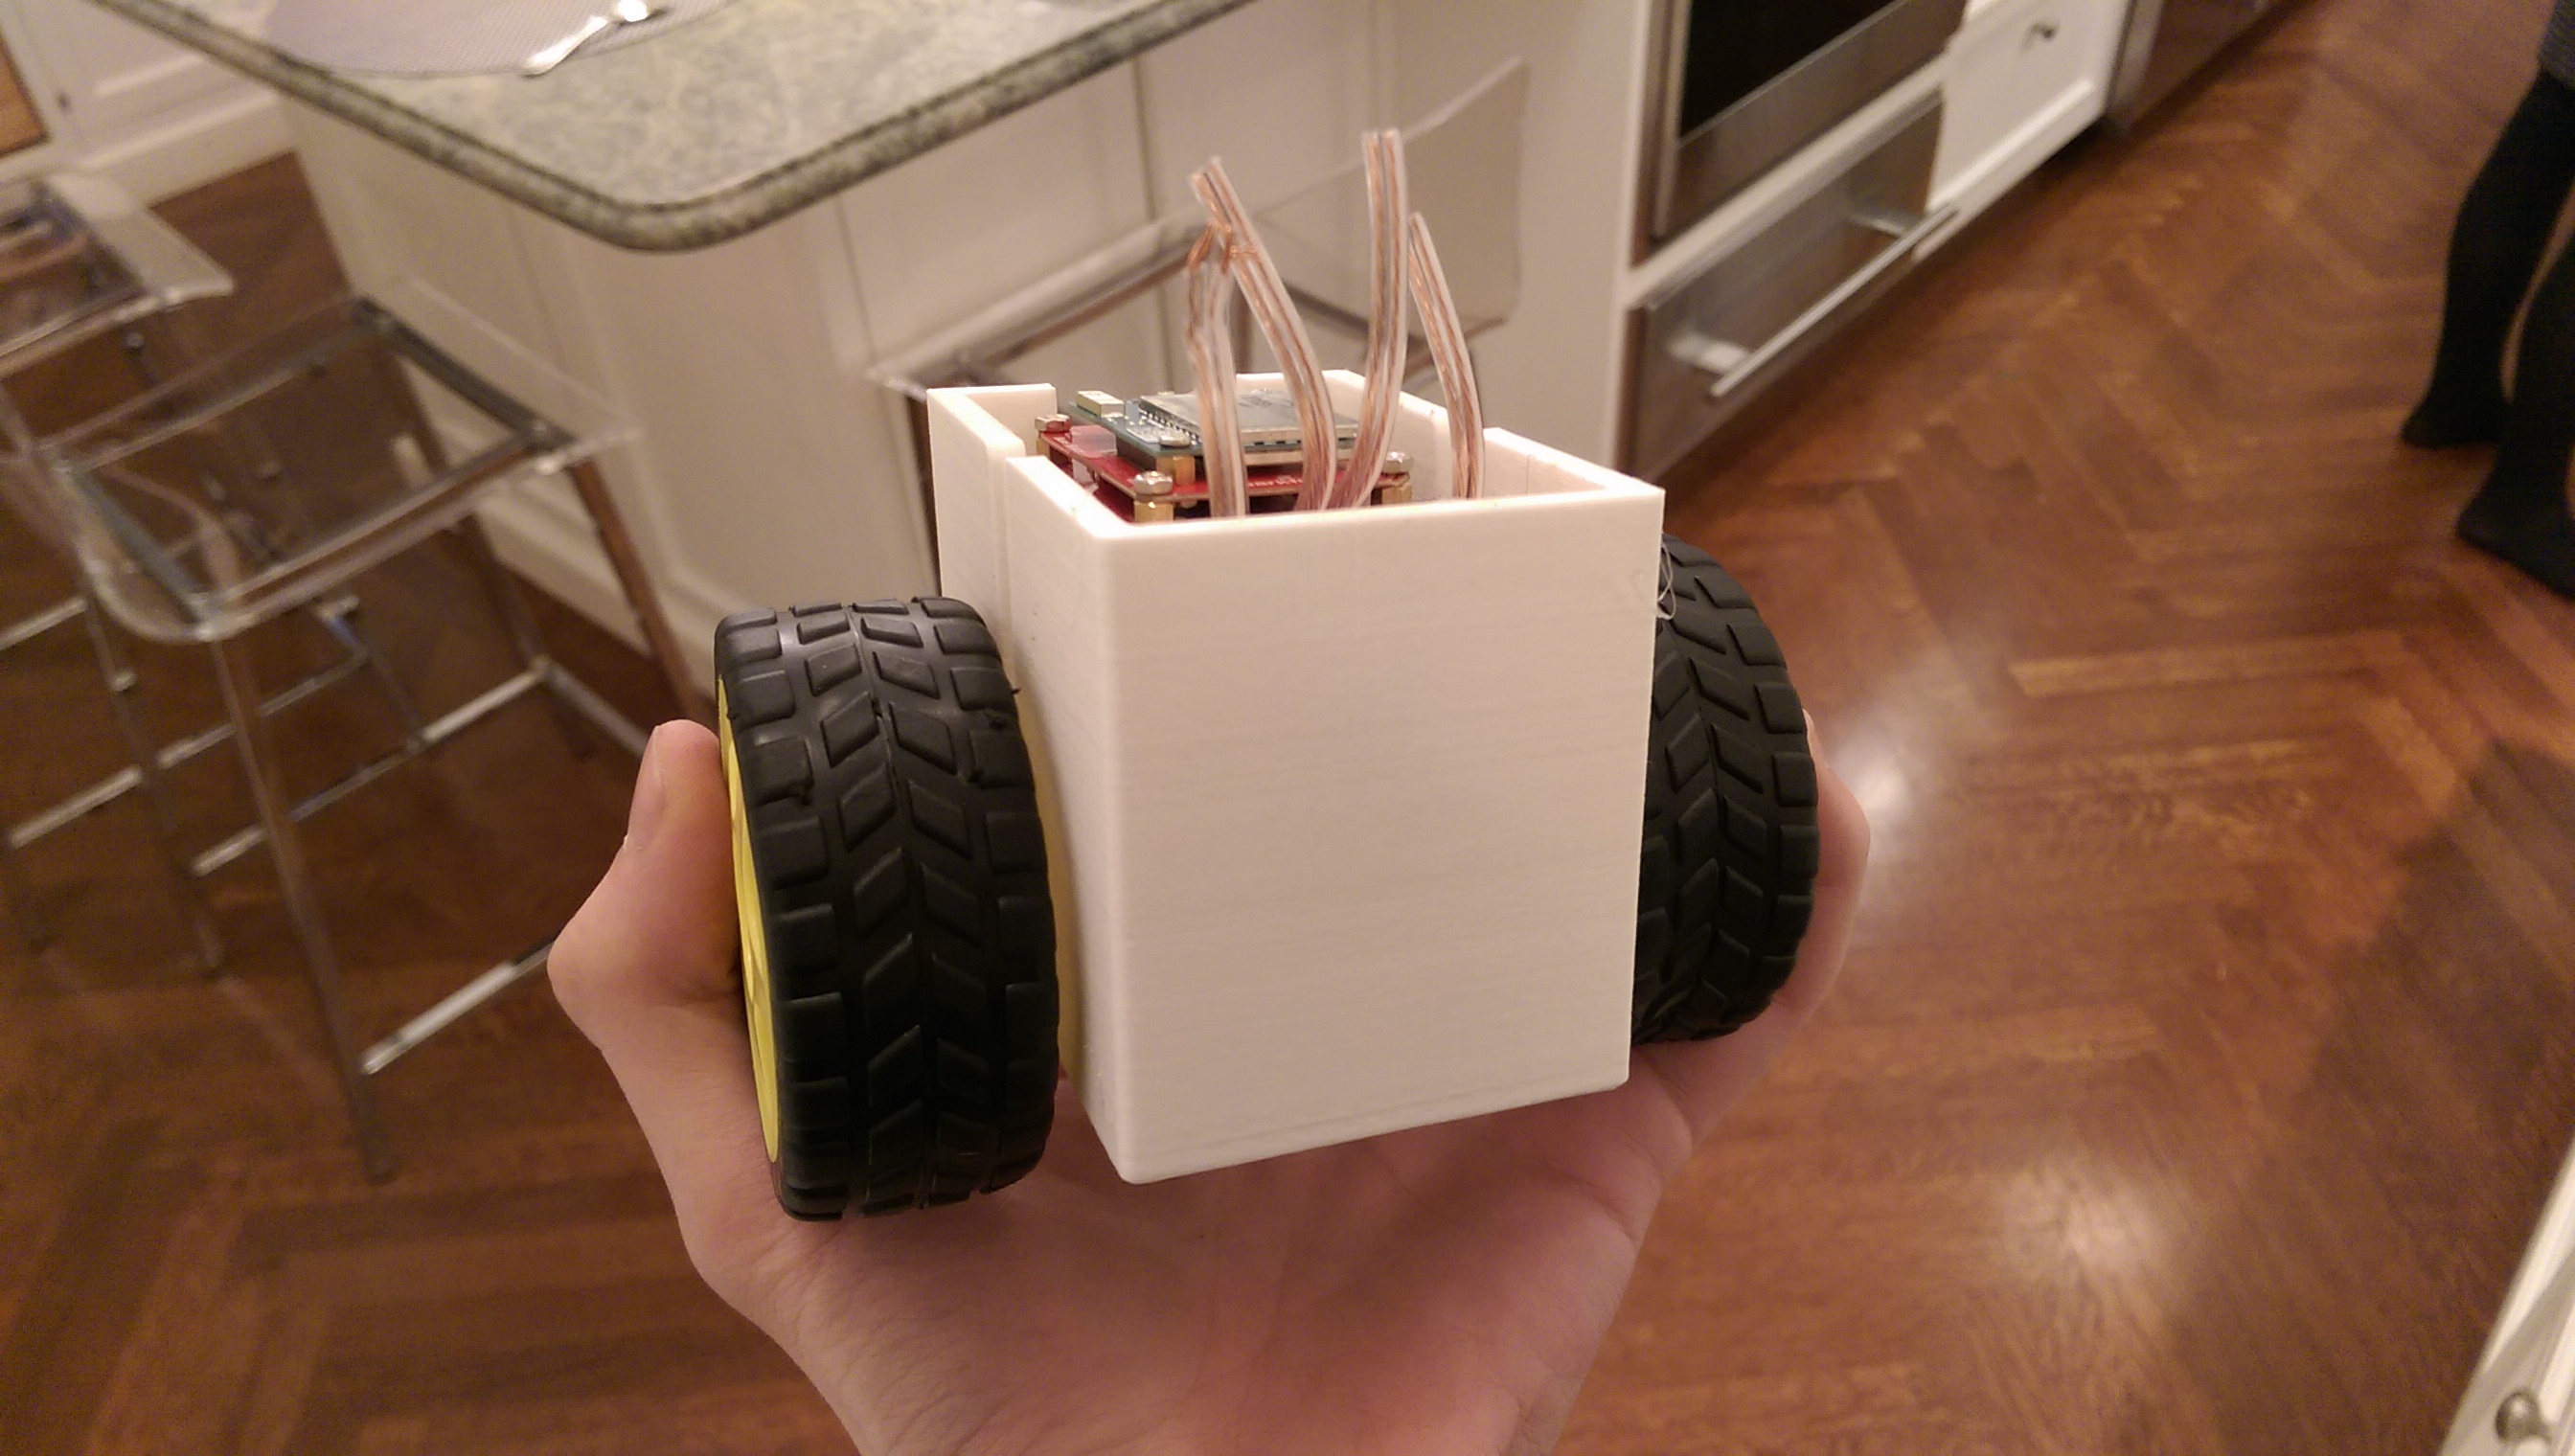
\includegraphics[width=.77\linewidth]{Figures/Prototype.jpg}
			\caption{Fido Hardware Implementation}
		\end{figure}
	\end{block}


\end{column}

\begin{column}{\sepwid}\end{column} 

\begin{column}{\twocolwid}

	\begin{block}{Learning Algorithm}
		\begin{columns}[t,totalwidth=\twocolwid]
			\begin{column}{\onecolwid}
				\begin{itemize}
					\item From a macro perspective, Fido can be viewed as a ``black box:'' inputs go in and outputs go out, Fido must optimize the relationship of inputs to outputs to maximize reward
					\item  \textbf{Reward system:} Trying to determine the expected reward for an action in a given state based on past reward received
					\begin{itemize}
						\item Must have a scalable, performance-optimized way of storing past state-reward sets and detecting patterns
					\end{itemize}
				\end{itemize}
			\end{column}
			\begin{column}{\onecolwid}
				\vspace{1cm}
				\begin{figure}
					\centering
					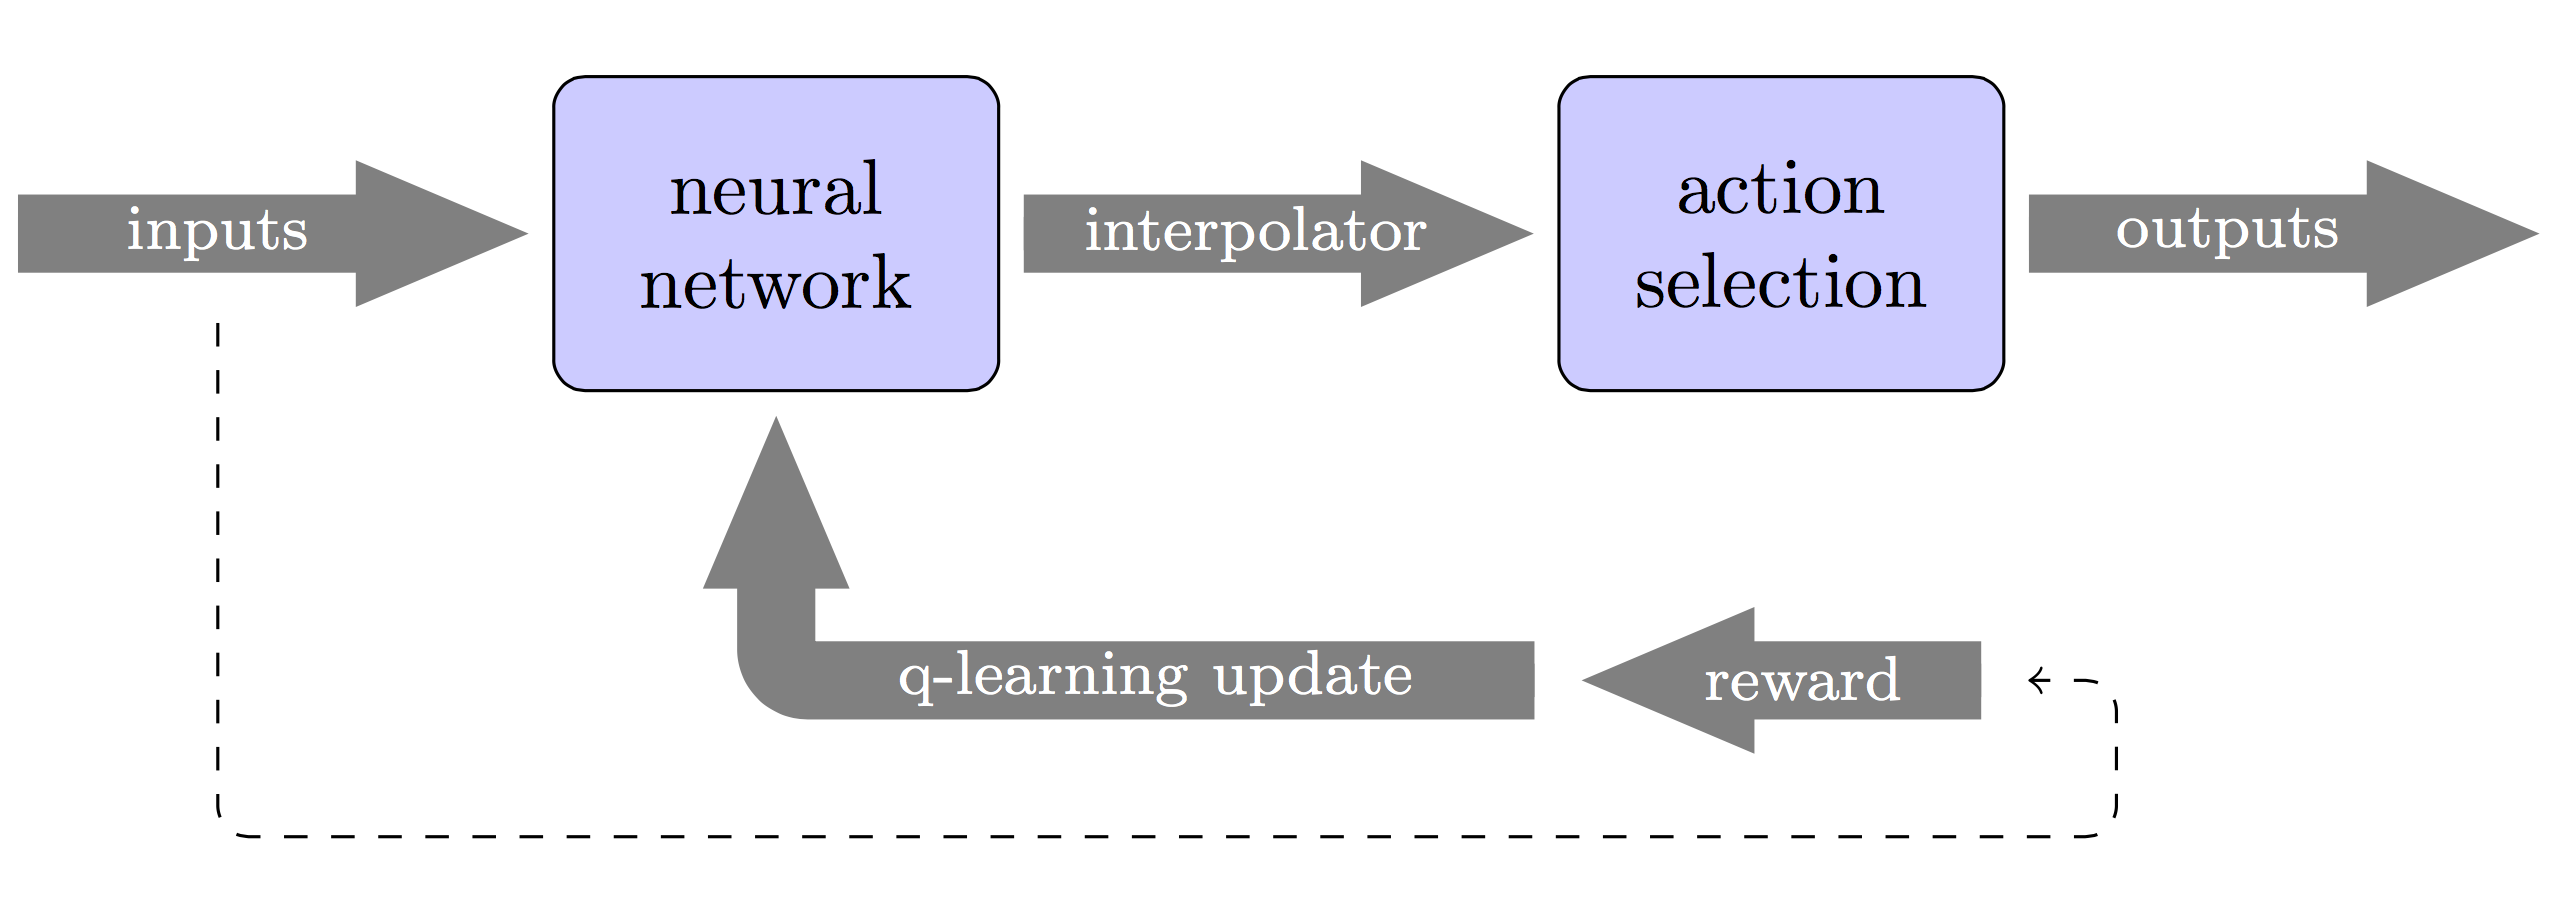
\includegraphics[width=\linewidth]{Figures/diagramRendered.png}
					\caption{Control System Diagram}
				\end{figure}
			\end{column}
		\end{columns}
	\end{block}

\begin{columns}[t,totalwidth=\twocolwid]

\begin{column}{\onecolwid}\begin{block}{Artificial Neural Networks}
	\begin{itemize}
		\item Function approximators modeled after nature with the capability to take in a large number of inputs, parallelly process them, and produce a set of outputs
	\end{itemize}
	\vspace{-1.2cm}
	\begin{figure}
		\centering
		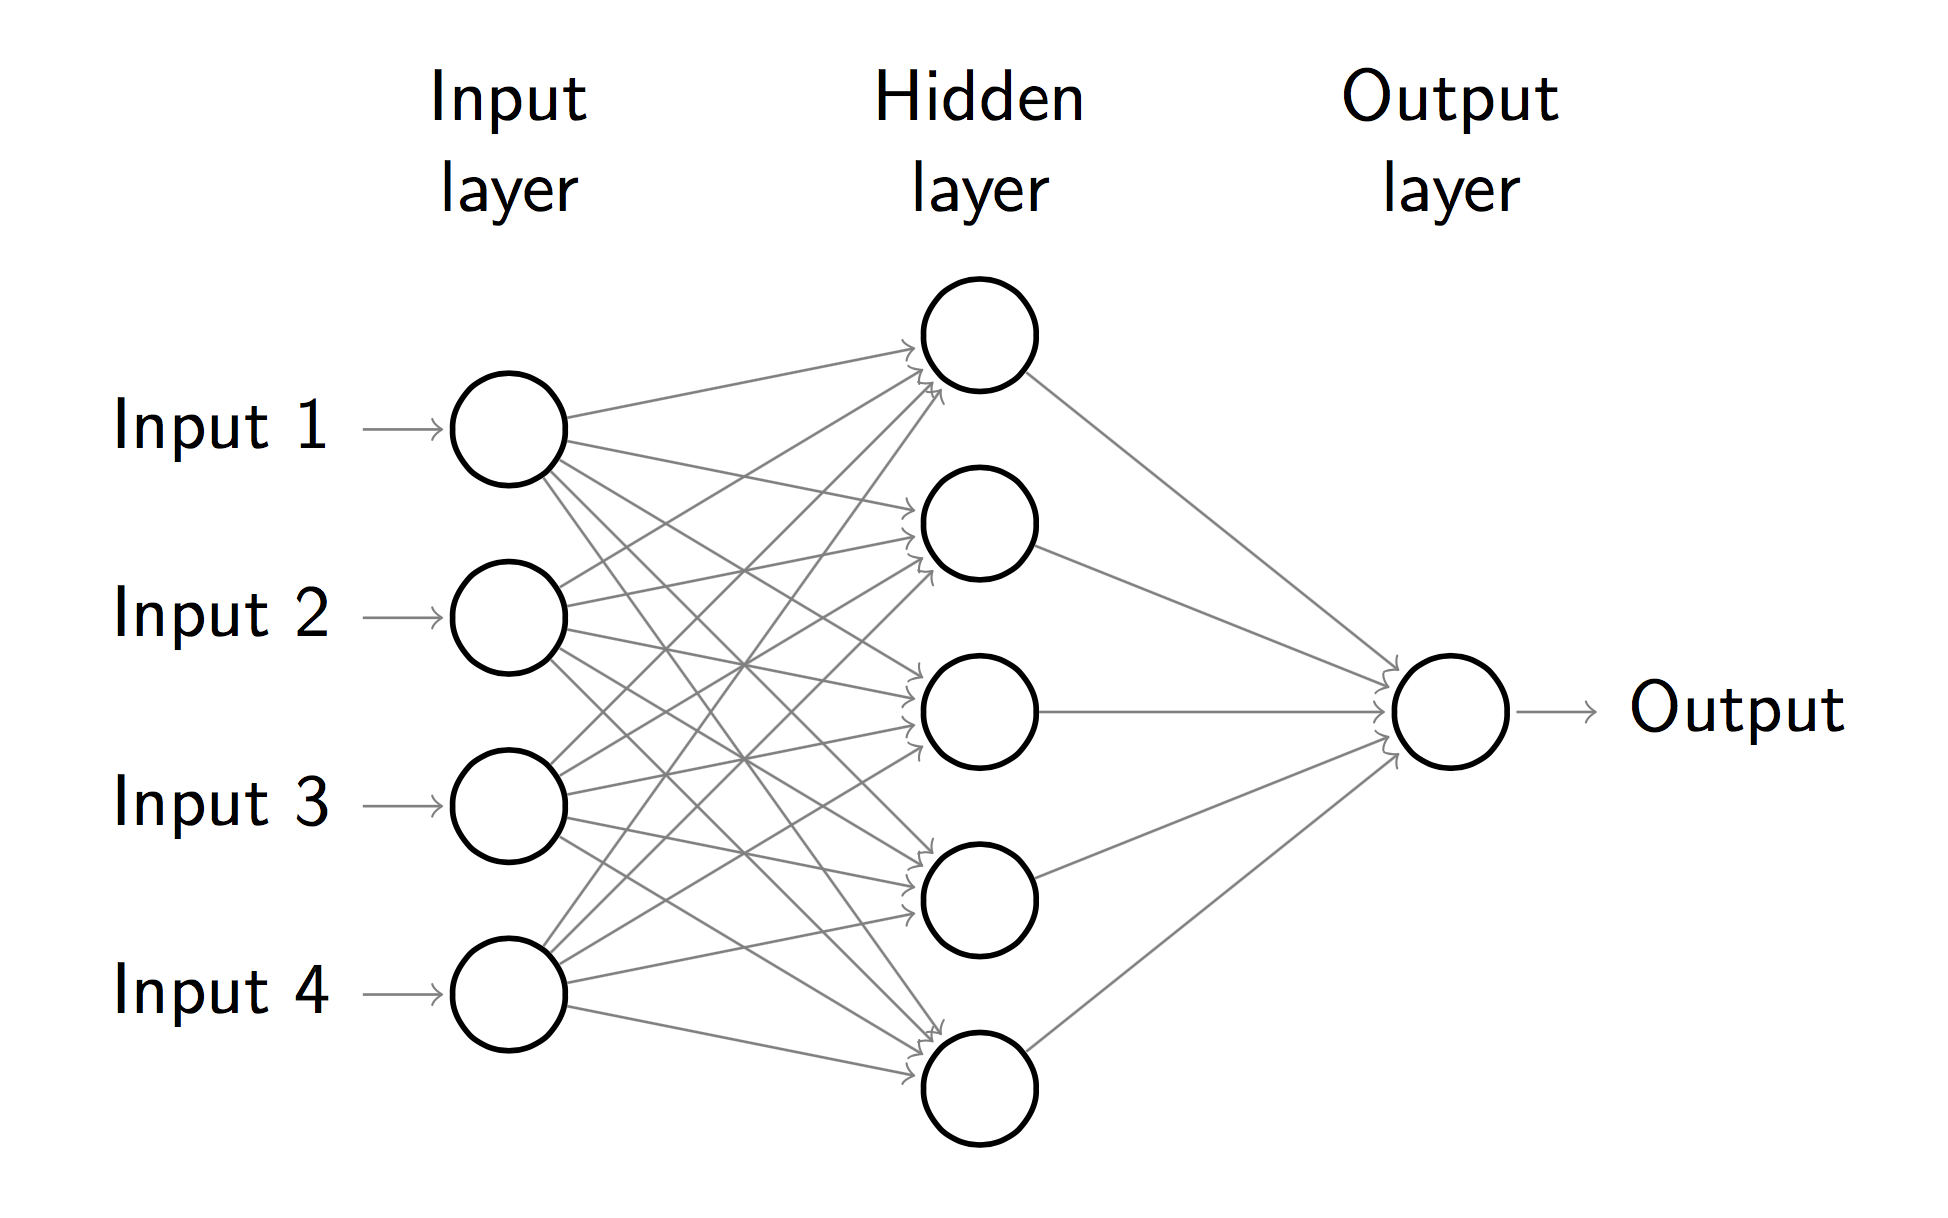
\includegraphics[width=.8\linewidth]{Figures/FeedForwardRendered}
		\caption{Single Output Feed-forward Neural Network}
		\label{fig:feedforward}
	\end{figure}
	\vspace{-3cm}
\end{block}\end{column}

\begin{column}{\onecolwid}\begin{block}{Reinforcement Learning}
	\begin{itemize}
		\item \textbf{Q-Learning:} Develops a function that intakes a state-action pair and outputs the expected utility
		\item Ordinarily the Q-function is modeled by storing state-action pairs in a table
		\begin{itemize}
			\item Is impractical for large state spaces, use a function approximator instead: \textbf{Artificial Neural Networks}
		\end{itemize}
		\item Usually discrete: no relation made between states or actions
		\begin{itemize}
			\item Can be optimized by coupling a wire-fitted interpolator with our neural network (\textbf{Wire-Fitted Q-Learning})
		\end{itemize}
		\item Cannot just pick the action with the greatest expected utility: must ``explore'' to be trainable and re-trainable
		\begin{itemize}
			\item Use a \textbf{Boltzmann Probability Distribution} selection policy
		\end{itemize}
	\end{itemize}


\end{block}\end{column} 

\end{columns} 

	\begin{block}{Results}
		Results were gathered both from simulation and hardware for a variety of tasks.  In simulation Fido was evaluated setting an LED  to measured light intensity (``Flash''), driving to a point with a direct XY-control drive system (``Float'') and a differential drive system (``Drive''), and line following.

		\begin{table}[ht]
			\centering
			\begin{tabular}{@{}lccc@{}}
				\toprule
				Task        & Learning Iterations & Action Selection (ms) & Training Time (ms) \\ \midrule
				Flash       & 6                   & 0.                  & 6               \\
				Float       & 14                  & 1                  & 6               \\
				Drive       & 17                  & 1                  & 11              \\
				Line Follow & 21                  & 2                  & 10.               \\ \bottomrule
			\end{tabular}
		\end{table}
		\vspace{.5cm}
		In hardware Fido was tasked with staying still and driving to a point.
		\begin{table}[ht]
			\centering
			\begin{tabular}{@{}lccc@{}}
				\toprule
				Task             & Learning Iterations & Action Selection (ms) & Training Time (ms) \\ \midrule
				Stay Still       & 3                   & 1                    & 43.5                  \\
				Drive to Point   & 18                  & 4                     & 65                  \\
			\end{tabular}
		\end{table}

	\end{block}

\end{column}

\begin{column}{\sepwid}\end{column}

\begin{column}{\onecolwid}

	\begin{block}{Future Development}
		We would like to experiment with dynamic optimization of hyperparameters, changing factors such as neural network architecture and Boltzman temperature constant to best fit the task at hand.  We also plan to package Fido as a machine learning library for embedded electronics and robotics, and build a microcontroller-based hardware implementation to further optimize for resource-limited environments.
	\end{block}

	\begin{block}{References}
		\nocite{*}
		\small{\bibliographystyle{IEEEtran}\bibliography{Poster}\vspace{0.75in}}
	\end{block}

	\setbeamercolor{block title}{fg=dblue,bg=white}
	\begin{block}{Acknowledgements}
		\small{\rmfamily{Thank you to Dr. Jeff Weitz of Horace Mann School, who gave us guidance in the art of scientific research.}}
	\end{block}

\end{column}

\end{columns}
\end{frame}
\end{document}

%%%%%%%%%%%%%%%%%%%%%%%%%%%%%%%%%%%%%%%%%
% Adapted from "Jacobs Landscape Poster" 
% (https://teamwork.jacobs-university.de:8443/confluence/display/CoPandBiG/LaTeX+Poster)
% License: CC BY-NC-SA 3.0 (http://creativecommons.org/licenses/by-nc-sa/3.0/)
%%%%%%%%%%%%%%%%%%%%%%%%%%%%%%%%%%%%%%%%%
